\documentclass{article}
\usepackage[a4paper, margin=2cm]{geometry}

\usepackage{amsmath}
\usepackage{amssymb}
\usepackage{mathtools}
\usepackage{amstext}
\usepackage{amsthm}
\usepackage{fancyhdr}
\usepackage{siunitx}
\usepackage{physics}
\usepackage{cancel}

\usepackage{hyperref}


\usepackage{graphicx}
\usepackage{float}
\graphicspath{{figures/}} %Setting the graphicspath
\usepackage{float}
\usepackage{caption}
\usepackage{subcaption}


\newcommand{\incfig}[2][1]{%
    \def\svgwidth{#1\columnwidth}
    \import{./figures/}{#2.pdf_tex}
}

\pdfsuppresswarningpagegroup=1

%\graphicspath{{figures/}}

\pagestyle{fancy}
\rhead{Alexandre Adam}
\lhead{PHY6669 -- Cosmologie \\ Alan Robinson}
\chead{Devoir 4}
\rfoot{\today}
\cfoot{\thepage}

\newcommand{\angstrom}{\textup{\AA}}
\numberwithin{equation}{section}
\renewcommand\thesubsection{\alph{subsection})}
\renewcommand\thesubsubsection{\Roman{subsubsection}}
\newcommand{\s}{\hspace{0.1cm}}

\newcommand{\hatp}{\hat{p}}

% Astronomy
\DeclareSIUnit\parsec{pc}
\DeclareSIUnit\lightyear{ly}

\begin{document}
\section{\textit{Dodelson} ch.4, Exercice 8}
On veut montrer que $T \propto a^{-2}$ lorsque $T$ représente la température (à l'équilibre)
de particules massives non-relativistiques sans interactions. Pour ce faire, 
on doit dériver l'équation de Boltzmann. On définit la direction 
du vecteur de quantité de mouvement $\hatp^{i}$ et la magnitude de la quantité de mouvement
\[
        p^2 \equiv  g_{ij} P^{i} P^{j}
\]
Par définition, la lettre majuscule $P$ réfère au 4-vecteur de la quantité de mouvement
\[
        P^{\alpha} \equiv\frac{d x^{\alpha}}{d \lambda} 
\]
Notons que
\[
        \delta_{ij}\hatp^{i}\hatp^{j} = 1
\]
de sortes que $\hatp^{i} = \hatp_{i}$. 

En supposant que $f= f^{(0)}$ est une distribution à l'équilibre, $f=f(E(p), t)$ ne 
peut que dépendre du temps et de la magnitude de la quantité de mouvement (ou de l'énergie dans notre cas). 
Aussi, 
le terme de collision $C[f] = 0$ par supposition de sortes que l'équation de Boltzmann est
\begin{equation}\label{eq:Boltzmann} 
        %\frac{d f(\mathbf{x}, p, \mathbf{\hatp}, t)}{d t} = \frac{\partial f}{\partial t} + 
        \frac{df(E, t)}{t} = 
        \frac{\partial f}{\partial t}
        %\frac{\partial f}{\partial x^{i}} \frac{d x^{i}}{d t} 
        %+ \frac{\partial f}{\partial \hatp^{i}} \frac{d \hatp^{i}}{d t} 
        + \frac{\partial f}{\partial E} \frac{d E}{d t} 
        =0
\end{equation} 
Pour poursuivre, on doit déterminer $\dfrac{dE}{dt}$. Notons que l'énergie remplace 
la quantité de mouvement $p$ pour le cas des photons (et se réduit à ce cas lorsque 
la particule a une masse nulle).
On travaille avec la métrique FRW
%perturbée, dans la jauge newtonienne conforme:
\begin{align*}
        g_{00} &=  -1 \\% - 2\Psi(\mathbf{x}, t) \\
        g_{0i} &= 0 \\
        g_{ij}(t) &=  a^2 \delta_{ij}%\left( 1 + 2 \Phi(\mathbf{x}, t) \right)
\end{align*}
Par définition, l'équation de conservation de l'énergie est
\[
        \frac{d P^{0}}{d \lambda} = -\Gamma^{0}_{\alpha \beta} P^{\alpha}P^{\beta} 
\]
On peut exprimer $P^{0}$ en terme de l'énergie en réalisant que 
\[
        P^2 = g_{\alpha \beta}P^{\alpha} P^{\beta} = -(P^{0})^2 + p^2 = -m^2
\]
d'où
\[
        P^{0} = \sqrt{p^2 + m^2} = E
\]
On utilise aussi la définition $P^{0} \equiv \dfrac{dt}{d\lambda}$, de sortes que 
multiplier $\dfrac{dP^{0}}{d\lambda}$ par $\dfrac{1}{P^{0}}$ revient à 
changer la variable $\lambda \rightarrow t$ dans la derivée:
\[
        \frac{1}{P^{0}}\frac{d P^{0}}{d \lambda} =
        \frac{dE}{dt} = 
        %\cancel{\frac{1}{E}} \frac{dp}{dt} = 
        %-\cancel{\frac{1}{E}}
        -\frac{1}{E}\Gamma^{0}_{\alpha \beta}P^{\alpha}P^{\beta}
\]
On se rappel que les seuls symbols de Christoffels temporels non-nuls sont 
$\Gamma^{0}_{ij} = \dfrac{da}{dt}a \delta _{ij} = a^2H \delta_{ij}$. Ainsi,
\[
        \frac{d E}{d t} = -\frac{a^2H}{E} \delta_{ij} P^{i}P^{j} 
\]
On écrit
\[
        P^{i} = C \hatp^{i}
\]
où $C$ est une constante de normalisation qu'on trouve avec la définition de $p^2$:
\[
        p^2 = C^2 a^2 \underbrace{\delta_{ij}\hatp^{i}\hatp^{j}}_{\equiv 1}
\]
puisque $\mathbf{\hatp}$ est un vecteur unitaire. Ainsi, $C = \dfrac{p}{a}$ et on trouve
\[
        \frac{d E}{d t} = -\frac{p^2H}{E} 
\]
L'équation de Boltzmann devient
\[
        \frac{\partial f}{\partial t} - \frac{p^2H}{E}\frac{\partial f}{\partial E} = 0
\]
Dans la limite non-relativiste, on peut prendre 
\[
        E(p) \simeq m + \frac{p^2}{2m}
\]
De sortes que 
\[
        \frac{p^2}{E} \frac{\partial f}{\partial E} \simeq \frac{p^2}{m} \frac{m}{p} \frac{\partial f}{\partial p}
\]
D'où
\[
        \frac{\partial f}{\partial t} - pH \frac{\partial f}{\partial p} = 0
\]
Pour déterminer le comportement de la température en fonction du facteur d'échelle, on 
suppose que $f$ est la distribution de Maxwell-Boltzmann:
\[
        f(p, t) \propto 
                \exp \left\{ -\frac{p^2}{2mT(t)} \right\}
\]
De sortes que,
\[
        \frac{\partial f}{\partial p} = f \left(-\frac{p}{mT}  \right)
\]
et
\[
        \frac{\partial f}{\partial T} = f \left( \frac{p^2}{2mT^2} \right)
\]
On trouve la relation
\[
        \frac{\partial f}{\partial T} = -\frac{p}{2T} \frac{\partial f}{\partial p}
\]
En remplaçant dans l'équation de Boltzmann, on obtient
\[
        \left( -\frac{1}{2T}\frac{d T}{d t} - \frac{1}{a}\frac{d a}{d t}   \right) p\frac{\partial f}{\partial E} = 0
\]
Ce qui est satisfait seulement lorsque
\[
        T \propto a^{-2}
\]

%%%%%%%%%%%%% DERIVATION dx/dt %%%%%%%%%%%%%%%%%%%%%%%%%%%%%%%%%%%55
%On cherche, en premier lieu, à determiner la forme de $\dfrac{dx^{i}}{dt}$. Pour ce faire, 
%on remarque que 
%\begin{align*}
        %P^{2} = g_{\alpha \beta} P^{\alpha}P^{\beta} &= m^2 \\
        %\implies -(1 + 2\Psi)(P^{0})^2 + p^2 &= -m^2 \\
        %\implies P^{0} &= \sqrt{m^2 + p^2}(1 - \Psi) \hspace{1cm} \{ \Psi \ll 1\} \\
%\end{align*}
%Selon notre approximation que la matière est non-relativistique, ceci revient à
%\[
        %P^{0} = m(1 - \Psi)
%\]
%Ceci nous permet d'écrire
%\[
        %\frac{d x^{i}}{d t} = \frac{d x^{i}}{d \lambda} \frac{d \lambda}{d t} = \frac{P^{i}}{P^{0}}
        %= \frac{P^{i}}{m}(1 + \Psi) 
%\]
%Sachant que (ceci suit de la définition de $p$ et $\hatp^{i}$)
%\[
        %P^{i} = \frac{p\hatp^{i}}{a}(1 - \Phi)
%\]
%On trouve
%\[
        %\frac{d x^{i}}{d t} = \frac{p \hatp^{i}}{a}(1 + \Psi - \Phi)
%\]



\section{Le faux vide}
\subsection{Densité de cordes cosmiques}
Une corde cosmique aurait une densité linéaire
\[
        \mu \simeq \frac{M^2}{\hbar c}
\]
Si on suppose que la distance typique entre deux cordes 
est de $100\,\,\mathrm{Mpc}$ alors la 
densité d'énergie est
\[
        \rho \simeq \frac{\mu}{(100\, \mathrm{Mpc})^{2}}
\]

\subsection{Les domaines cosmologiques}
%Un domaine où la phase d'un champ scalaire $\phi$ est constante forme 
%un mur avec une densité surfacique
%\[
        %\eta \sim \frac{M^3}{(\hbar c)^2}
%\]
Si on suppose que ce mur possède une coordonnée comobile constante, alors 
son énergie est équivalente à son énergie de masse $E \sim \rho V$. 
La pression exercée par ce mur est 
\[
        P = - \frac{d E}{d V} = -\rho
\]
De sortes que
\[
        \boxed{w \sim \frac{\rho}{P} \sim -1}
\]
\section{\textit{Dodelson} ch.6, Exercice 4}
\subsection{\textit{Flatness problem}}
Le \textit{flatness problem} stipule est la réalisation que le paramètre de courbure 
$\kappa$ est très proche de 0 (Univers plat), 
ce qui requiert en principe une condition initiale 
très précise pour $\Omega$. On exprime le paramètre de courbure en terme du paramètre de densité 
d'énergie totale dans l'Univers $\Omega$:
\[
        1 - \Omega(t) = -\frac{\kappa}{a^2(t) H^2(t)}
\]
Lorsque $a(t) \rightarrow 0$, le côté droit de l'équation $\rightarrow \infty $ si $\kappa \not= 0$, 
de sortes que si le côté gauche est différent de $0$ lors des premiers moments de l'Univers, 
$\kappa$ va devoir prendre une valeur absolue très grande $|\kappa| \gg 1$ pour compenser 
la petitesse du paramètre d'échelle. On peut visualiser le comportement du côté droit 
en posant $\Omega_{0} = \Omega_{r,0} + \Omega_{m,0} = 0.3$:
\[
        \Omega(t) \equiv \frac{8 \pi G \rho(t)}{3H^2(t)}
\]
où $\rho$ est la densité d'énergie de la radiation et de la matière. On pose que
\[
        H^2(t) = H_0^2 \left( \Omega_{r,0}a^{-4} + \Omega_{m,0}a^{-3}  + (1 - \Omega_0)a^{-2} \right)
\]
Où $\Omega_0$ est la valeur du paramètre de densité total observé aujourd'hui. On a négligé le 
paramètre d'énergie sombre pour simplifier l'argument.
On a que
\[
        \rho(t) = \Omega_{m, 0}\rho_{\mathrm{crit}}a^{-3} + \Omega_{r,0}\rho_{\mathrm{crit}}a^{-4}
\]
De sortes que
\[
        \Omega(t) = \frac{\Omega_{m, 0}a + \Omega_{r,0}}{\Omega_{r, 0} + \Omega_{m, 0}a + (1 - \Omega_0)a^{2}}
\]
et 
\[
        1 - \Omega(t) = \frac{(1 - \Omega_0)a^{-2}}{\Omega_{r, 0} + \Omega_{m,0}a + (1 - \Omega_0)a^{2}}
\]
Naturellement, lorsque $a \rightarrow 0$, la valeur précise de $\Omega_0$ importe 
peu et $|1 - \Omega(t)| \rightarrow 0$.
\begin{figure}[H]
        \centering
        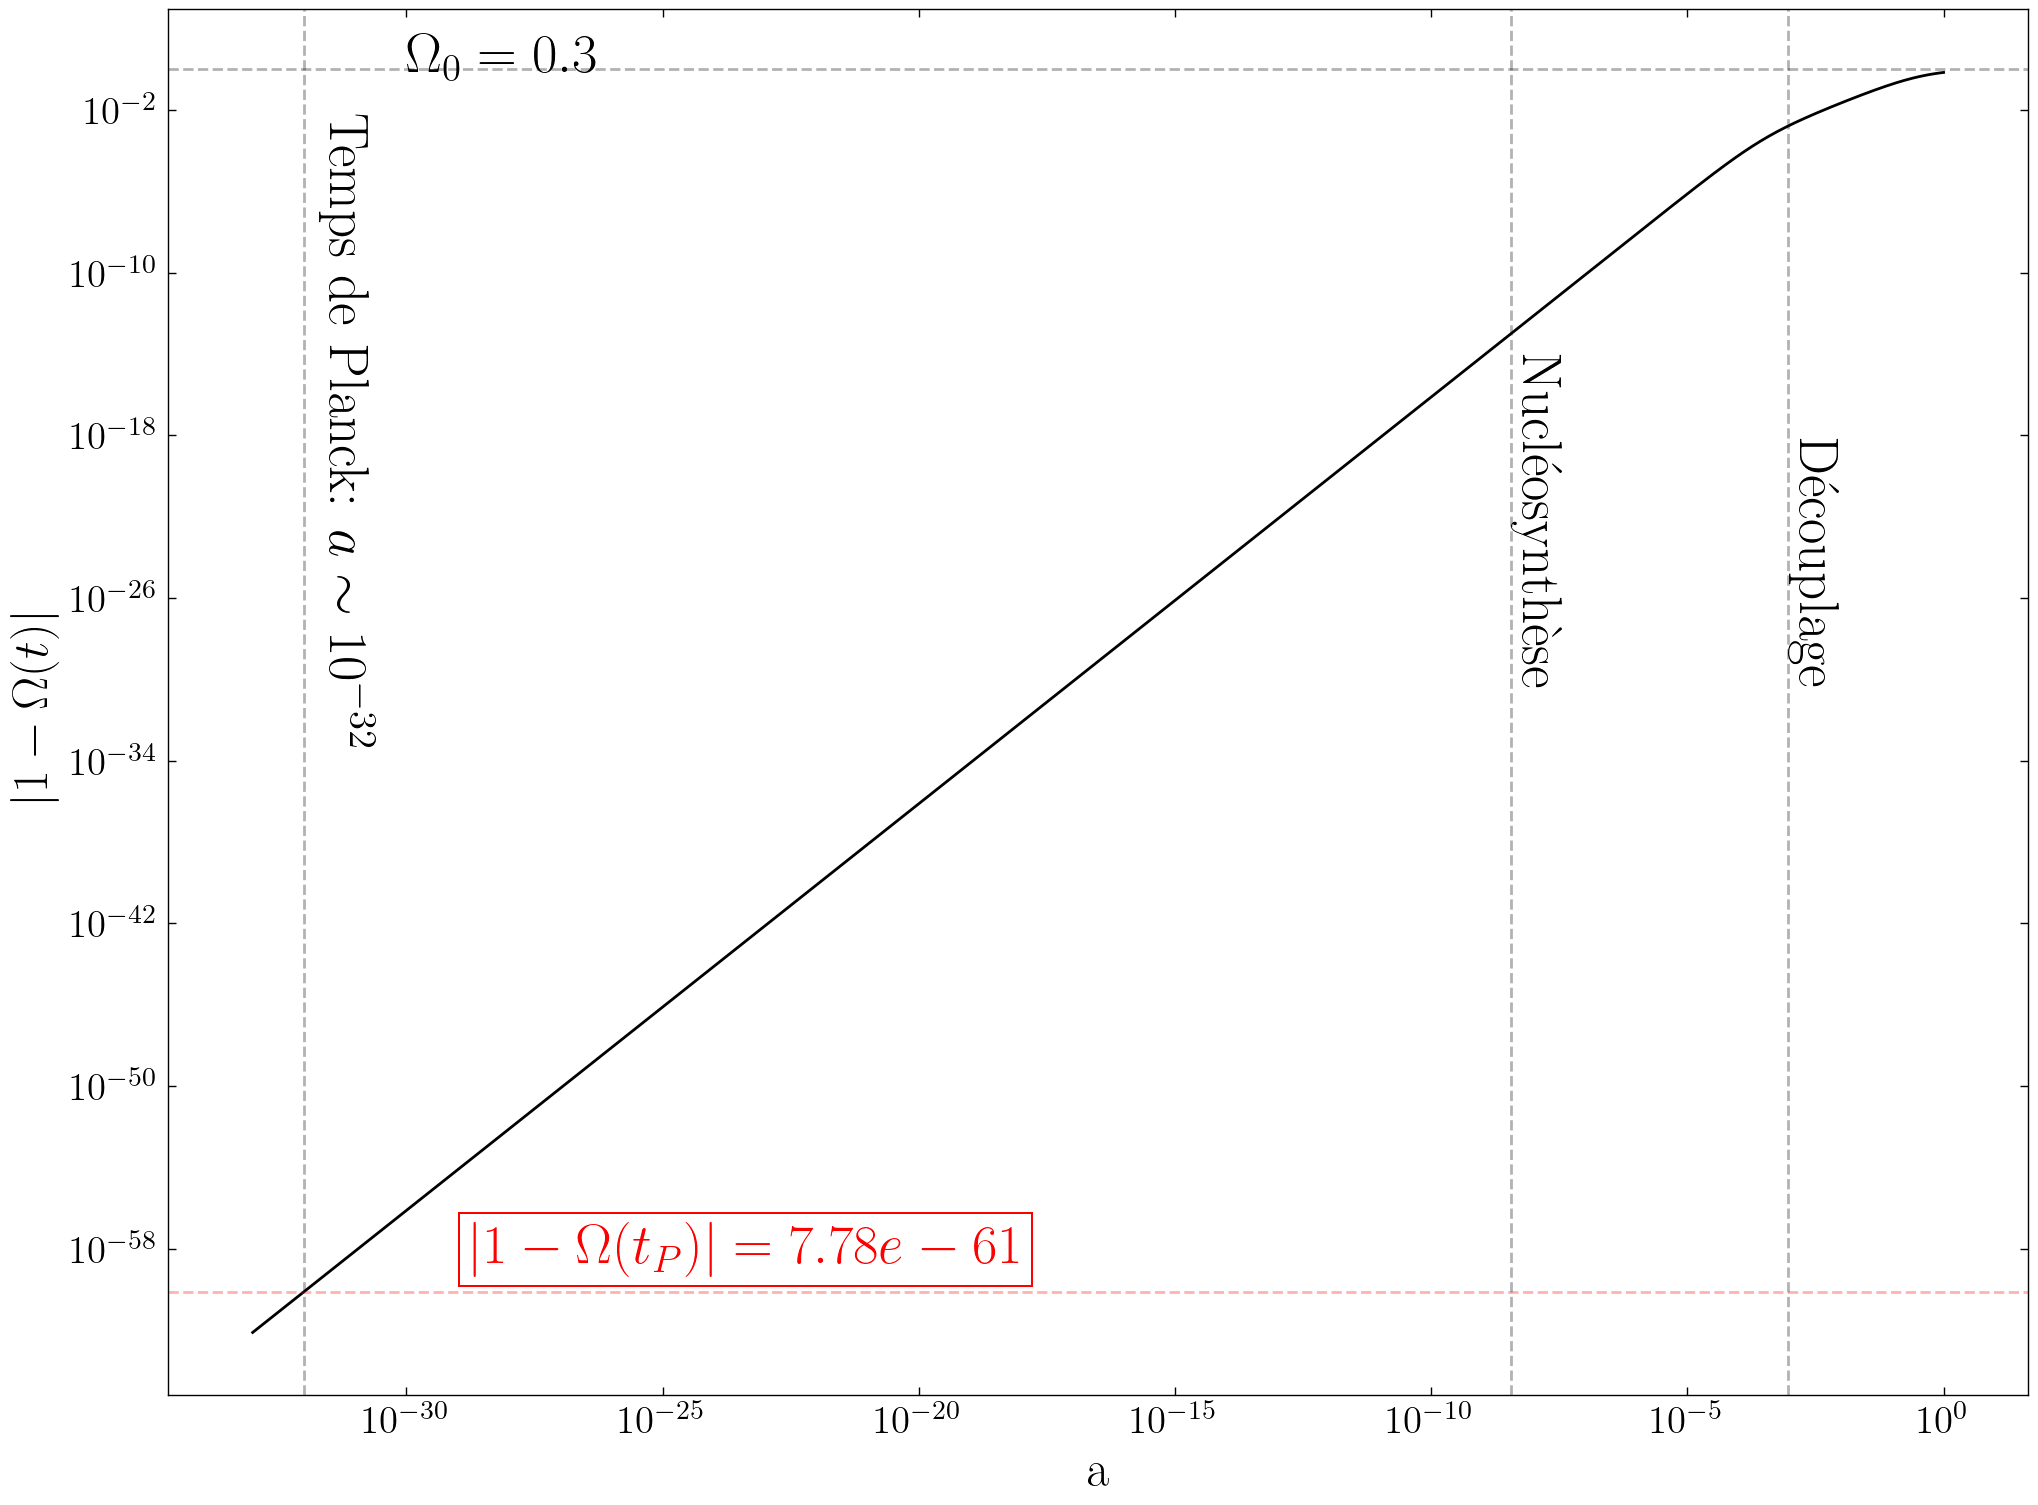
\includegraphics[width=0.8\textwidth]{omega}
        \caption{Paramètre de densité au début de l'Univers.}
\end{figure}

\subsection{Inflation}
L'inflation est une époque dans l'univers où l'accélération de l'expansion $\ddot{a} > 0$. 
La seconde équation de Friedmann s'écrit
\[
        \frac{\ddot{a}}{a} = \frac{\Lambda_i}{3} > 0 
\]
où on a supposé que l'équation d'état de cette énergie du vide est $P = -\rho/3$. Cette équation 
différentielle a comme solution
\[
        a(t) \propto e^{H_i t}
\]
où $H_i$ est la constante de Hubble durant l'inflation (constante en fonction du temps). Ainsi, 
durant l'inflation, on a
\[
        1 - \Omega(t) \propto \frac{1}{H_i}(1 - \Omega_0)e^{-2H_i t}
\]
Si on pose $t_i$ comme le temps au début de l'inflation et $t_f$ le temps à la fin, alors
\[
        |1 - \Omega(t_f)| = e^{-2N}|1 - \Omega(t_i)|
\]
où $N$ est le nombre de repliements exponentiels ayant eu lieu durant l'inflation $t_f \simeq (N + 1)t_{\mathrm{GUT}}$.
Si 
$N$ est suffisamment grand, alors la valeur de $\Omega(t_i)$ n'a plus besoin d'être aussi 
proche de 1, comme dans le cas étudié au sous numéro précédent. En particulier, 
on peut choisir $\Omega(t_{\mathrm{GUT}}) = 0$ pour une inflation qui perdure durant $N=60$ repliement 
exponentiels. 
\[
        a_{\mathrm{GUT}} \simeq \frac{T_{\mathrm{CMB}}}{T_{\mathrm{GUT}}} \simeq 2.73\times 10^{-28}
\]
On peut déterminer $a(t_f)$, soit le facteur d'échelle après l'inflation à partir de la valeur de $N$ 
choisit
\[
        \boxed{a(t_f) \simeq a_{\mathrm{GUT}}\sqrt{N + 1}}
\]
puisque $a \sim t^{1/2}$ dans l'Univers jeune. On utilise cette valeur pour extrapoler la valeur de 
$|1 - \Omega(t)|$ avant et durant l'inflation.
\begin{figure}[H]
        \centering
        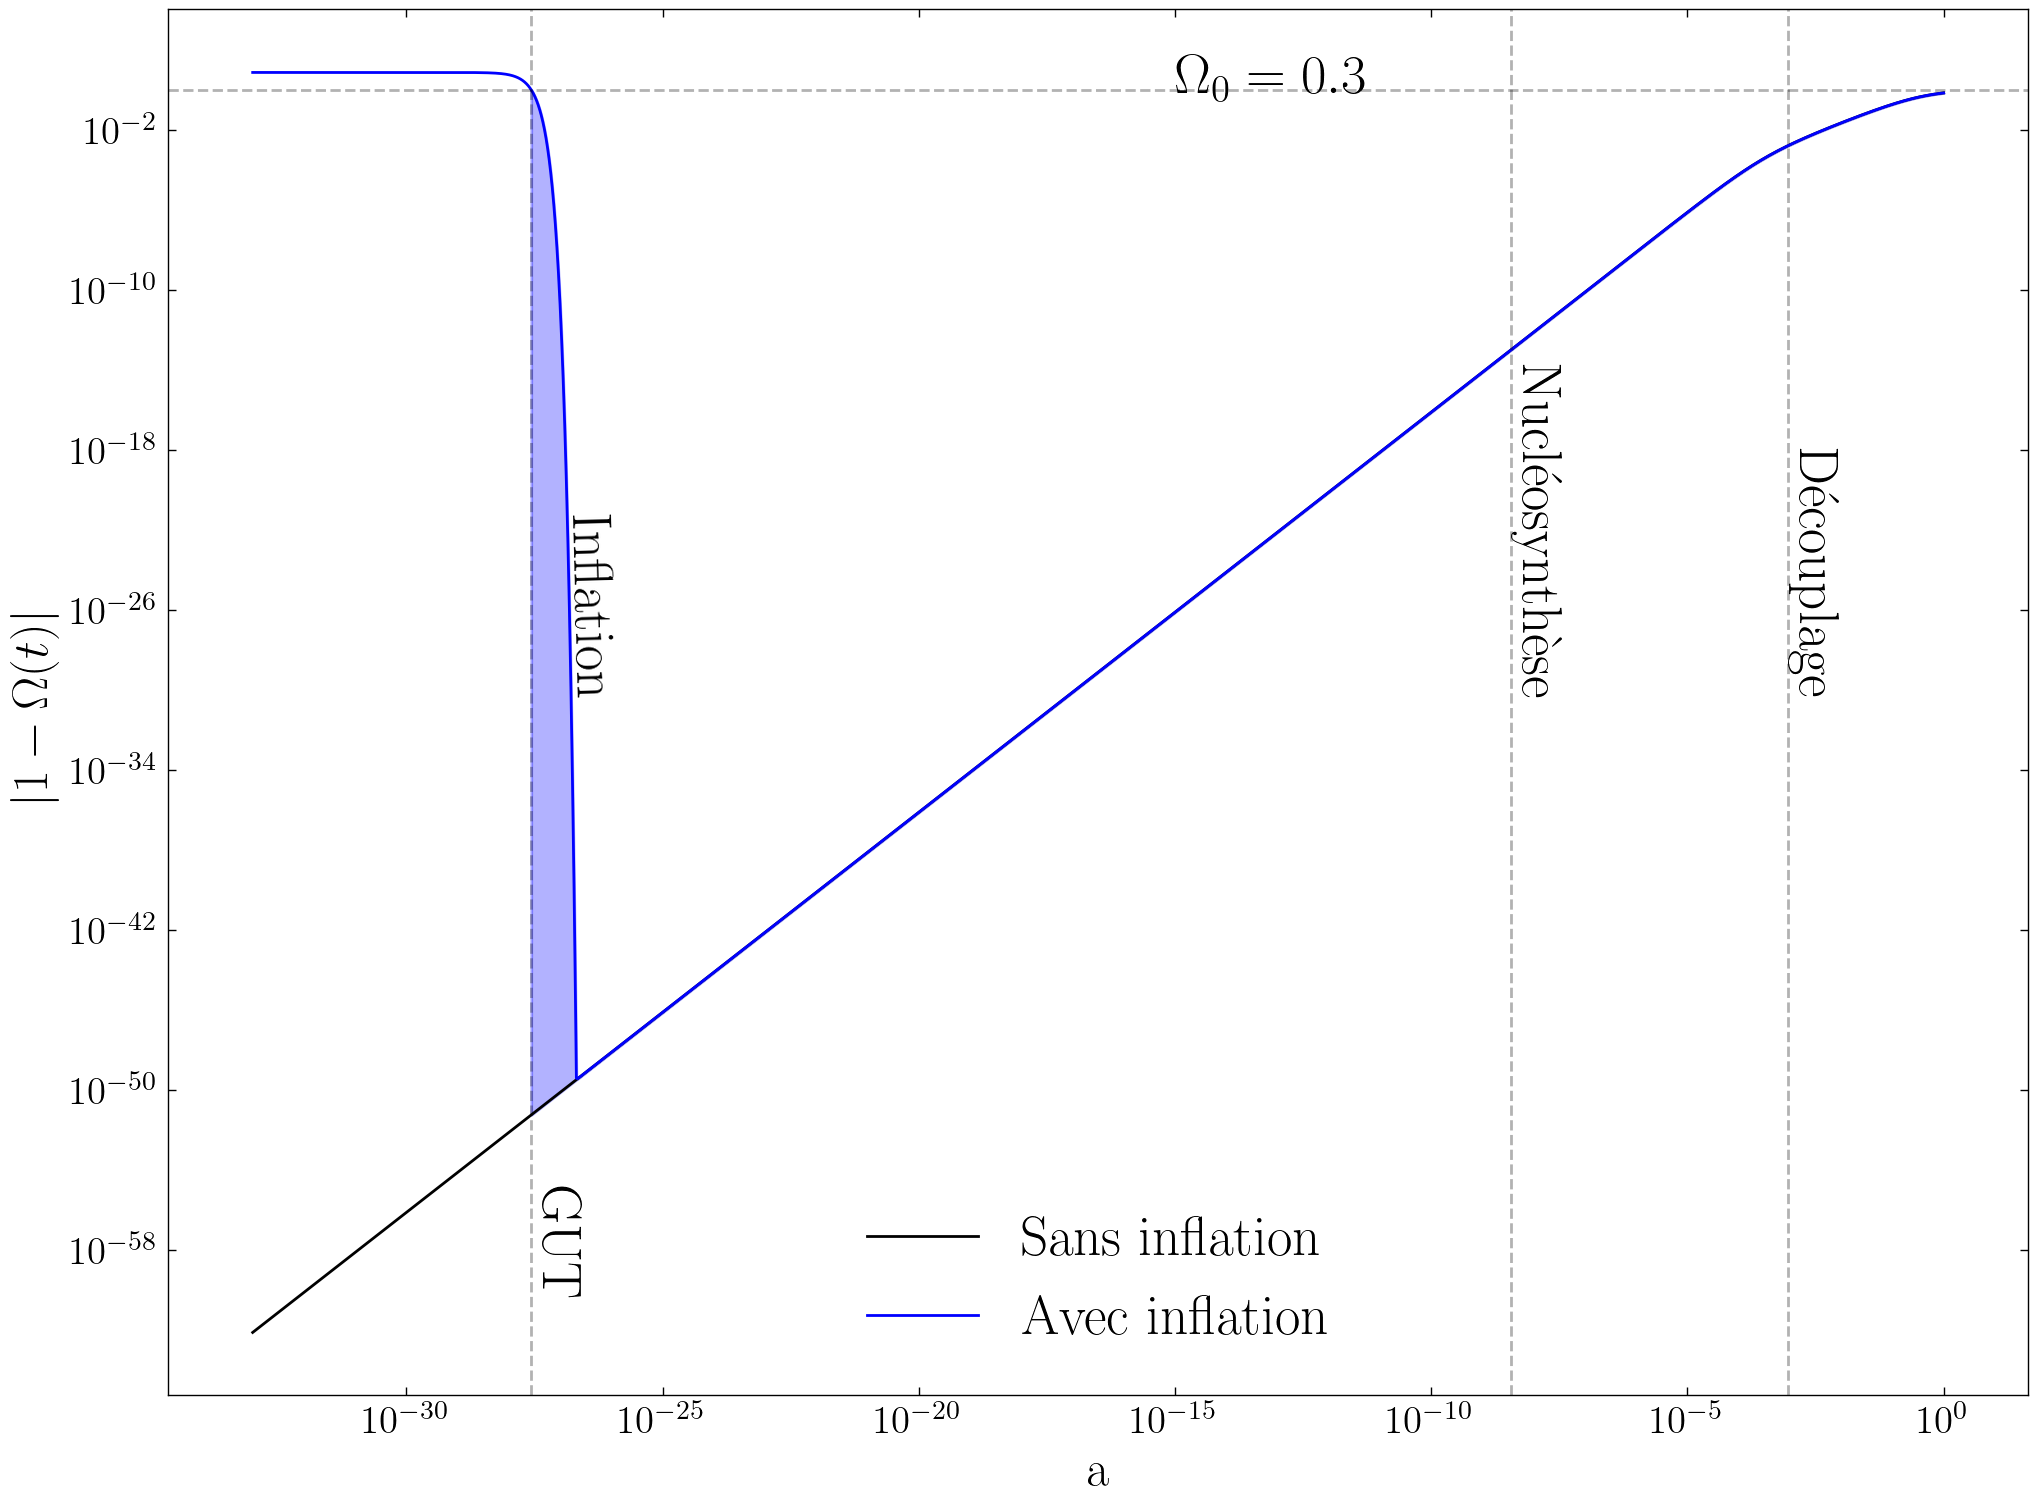
\includegraphics[width=0.8\textwidth]{omega_inflation}
        \caption{L'inflation fait en sortes que $\Omega(t_i)$ peut prendre n'importe quelle valeur, et 
        les observations faites aujourd'hui sont respectées.}
\end{figure}






\end{document}

